\documentclass{article}
\usepackage{graphicx}

\title{Cara Membuat Aplikasi Oracle Apex}
\author{nurulkamila1899 }
\date{October 2019}

\begin{document}

\maketitle

\section{Buka Oracle Apex, lalu masukkan workspace, username beserta password dan sign in}
\begin{center}
    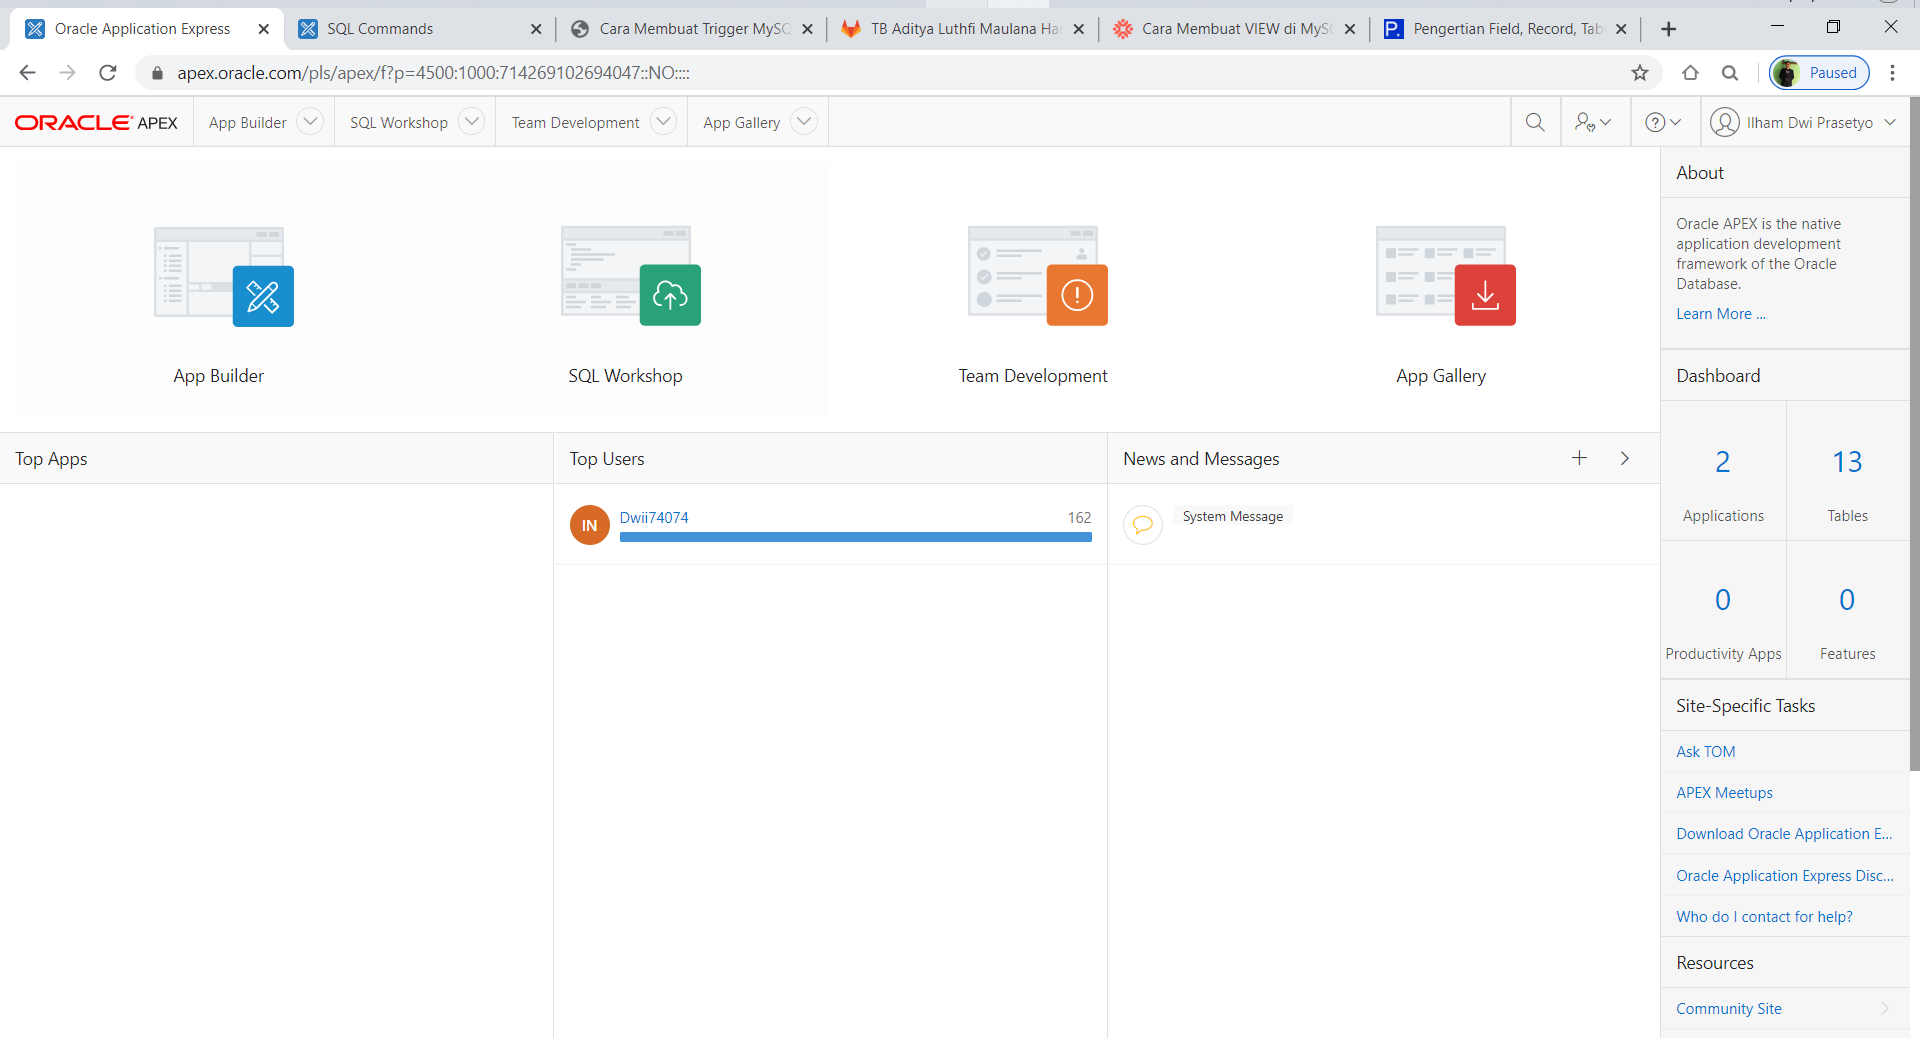
\includegraphics[width=.8\textwidth]{1.PNG}
\end{center}
\section{Jika sudah masuk, klik App Builder}
\begin{center}
    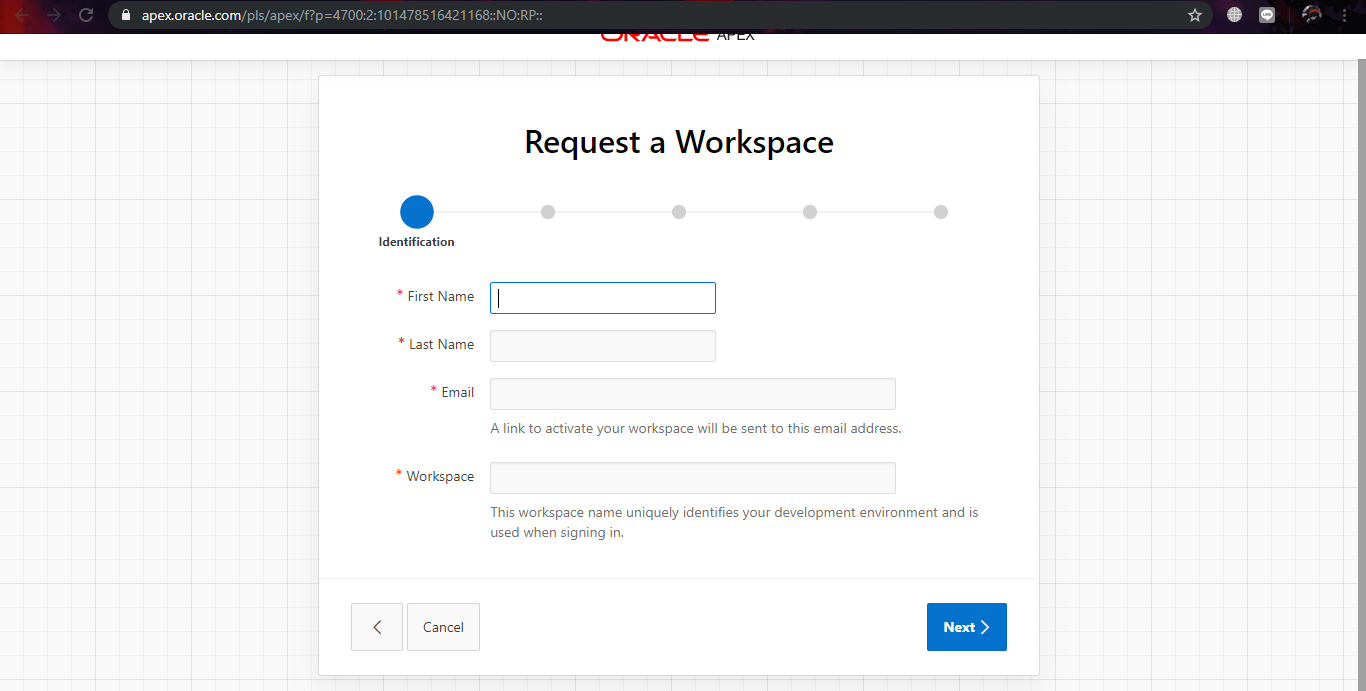
\includegraphics[width=.8\textwidth]{2.PNG}
\end{center}
\section{Selanjutnya klik Creat}
\begin{center}
    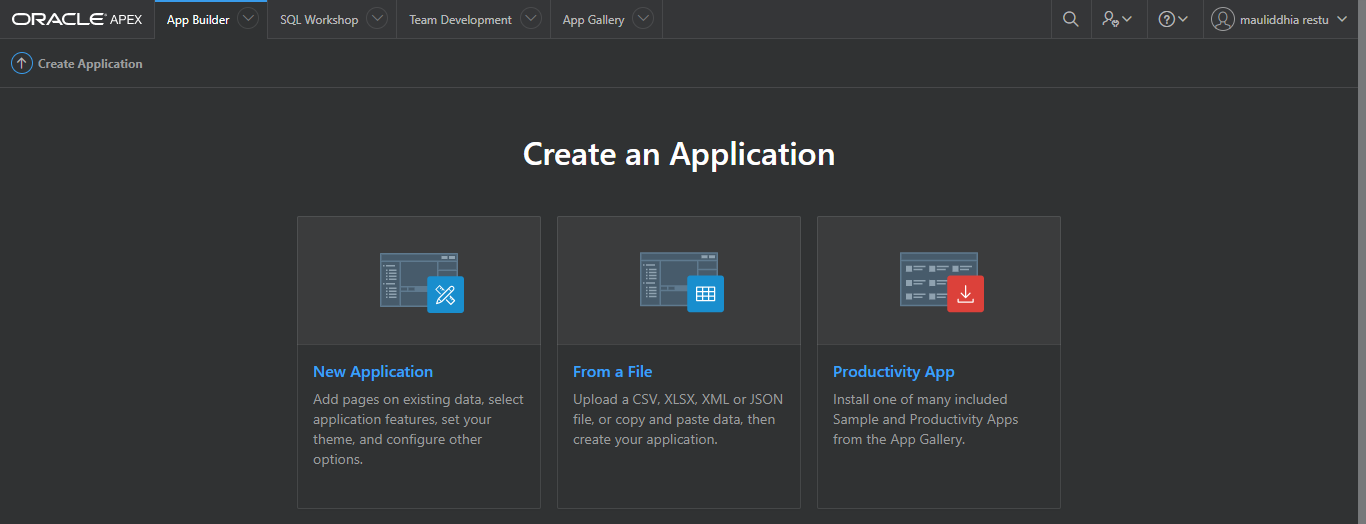
\includegraphics[width=.8\textwidth]{3.PNG}
\end{center}
\section{Pada laman Creat an Application, pilih Form a File}
\begin{center}
    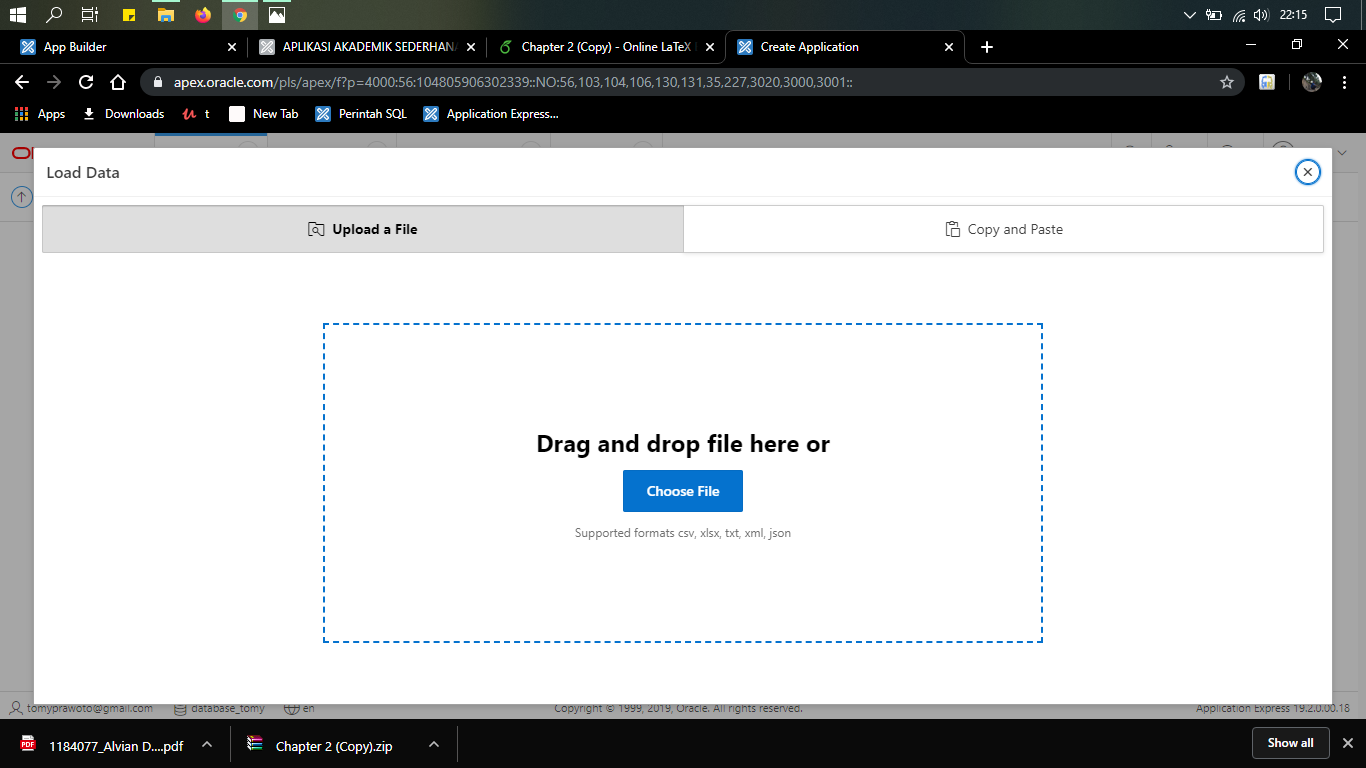
\includegraphics[width=.8\textwidth]{4.PNG}
\end{center}
\section{Lalu, klik Choose File dan pilih file exel yang berisikan data , seperti contoh di bawah ini yaitu data mahasiswa}
\begin{center}
    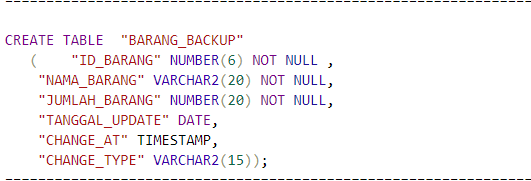
\includegraphics[width=.8\textwidth]{5.PNG} \\
    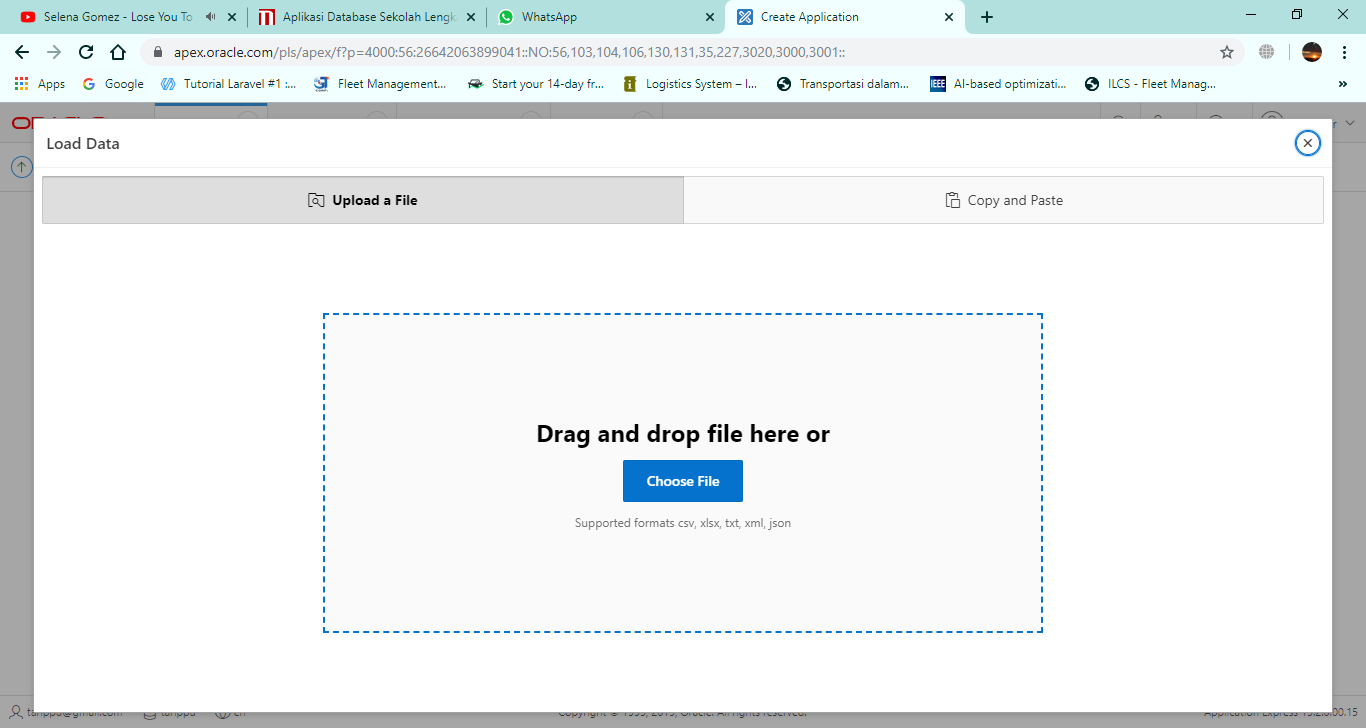
\includegraphics[width=.8\textwidth]{6.PNG}
\end{center}
\section{Pada laman selanjutnya, silahkan masukkan nama Table sesuai yang kamu inginkan, perlu diketahui pada kolom error table name akan terisi otomatis. Lalu klik Load Data maka data tersebut akan di import ke oracle.}
\begin{center}
    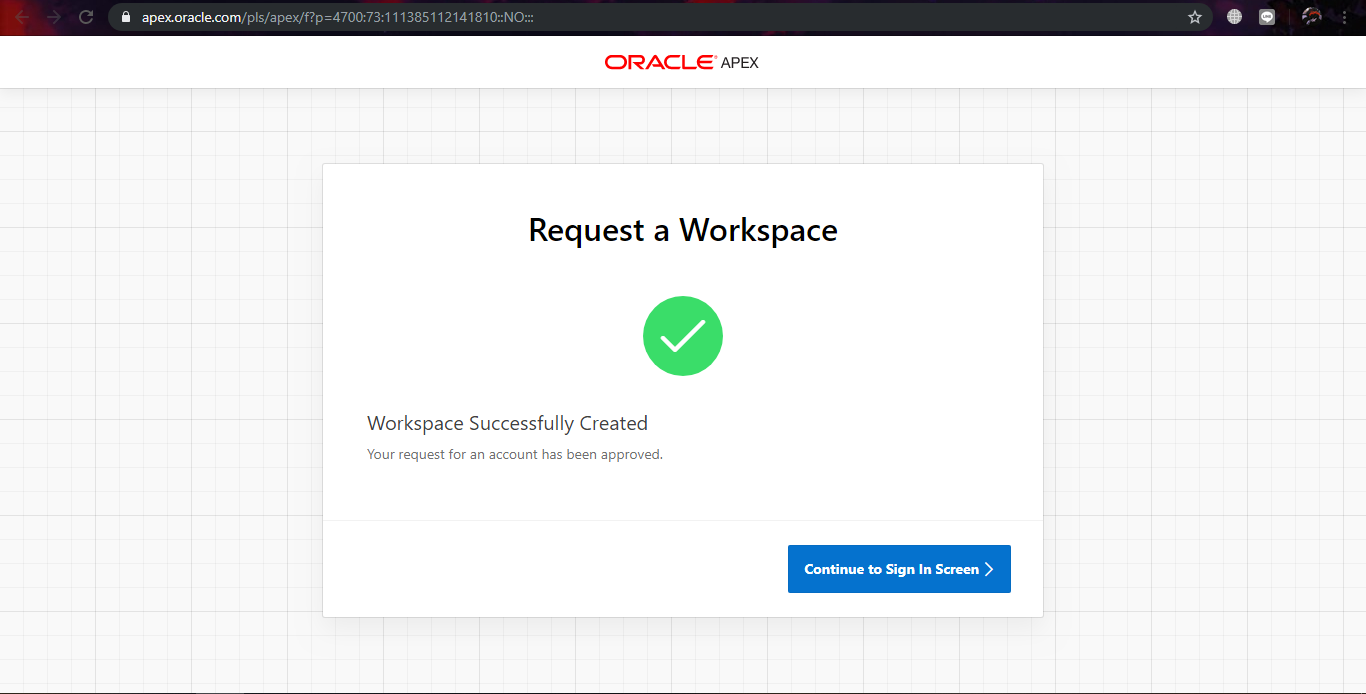
\includegraphics[width=.8\textwidth]{7.PNG} \\
    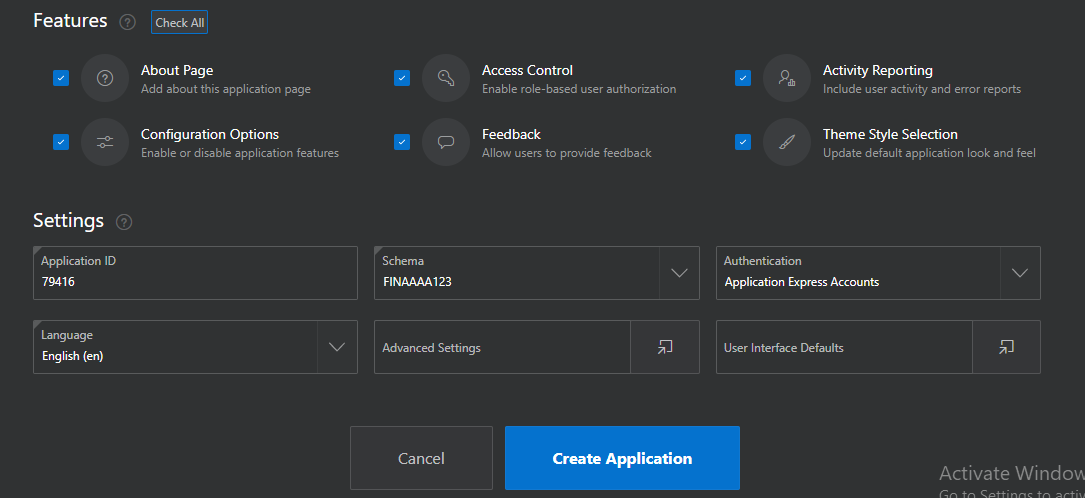
\includegraphics[width=.8\textwidth]{8.PNG}\\
    Klik creat Application
\end{center}
\section{Pada laman selanjutnya, scroll kebawah dan centang semua menu pada Features, lalu pilih Creat Application}
\begin{center}
    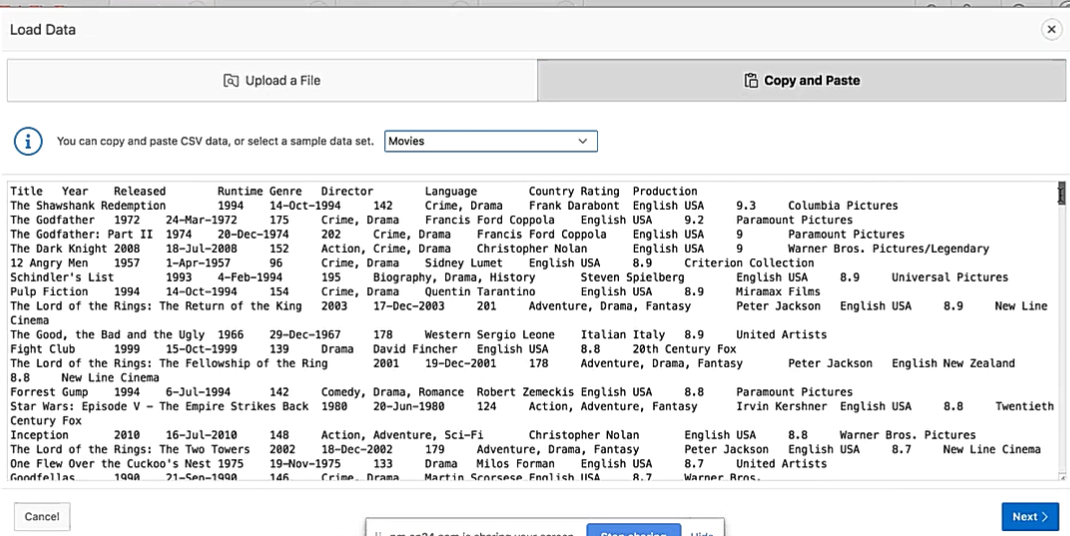
\includegraphics[width=.8\textwidth]{9.PNG} \\
    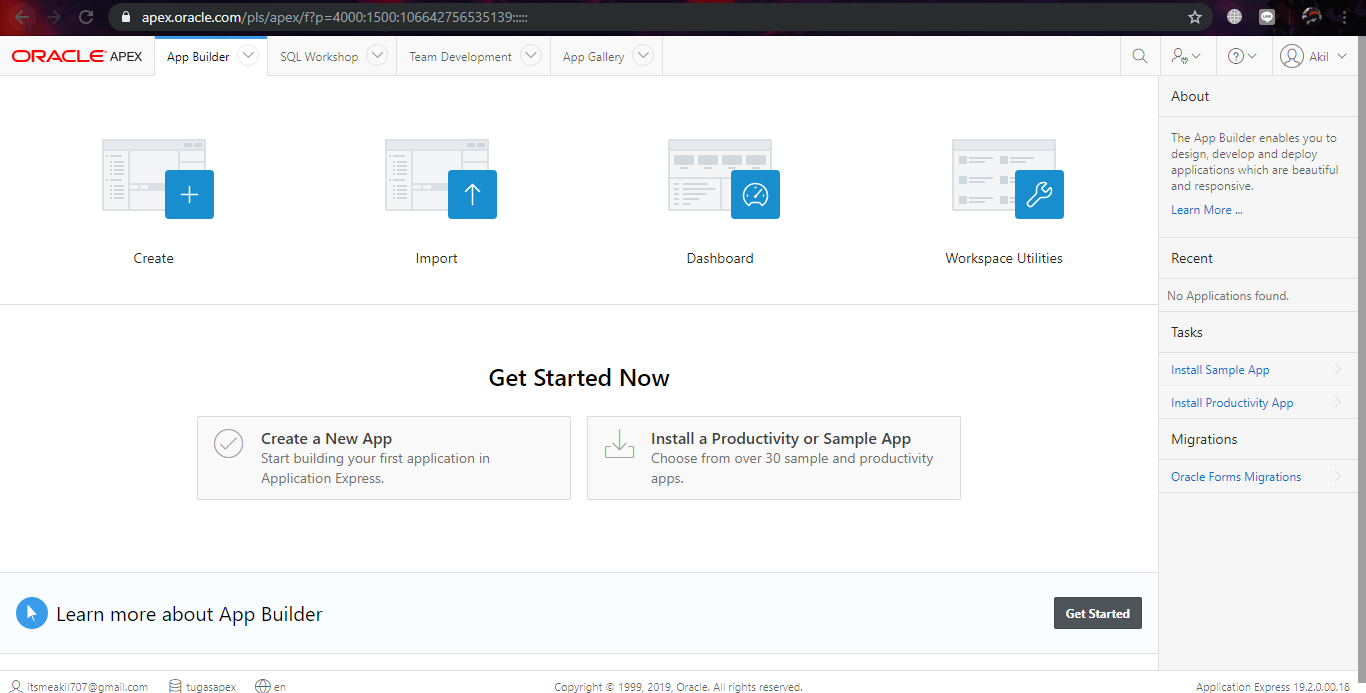
\includegraphics[width=.8\textwidth]{10.PNG} \\
    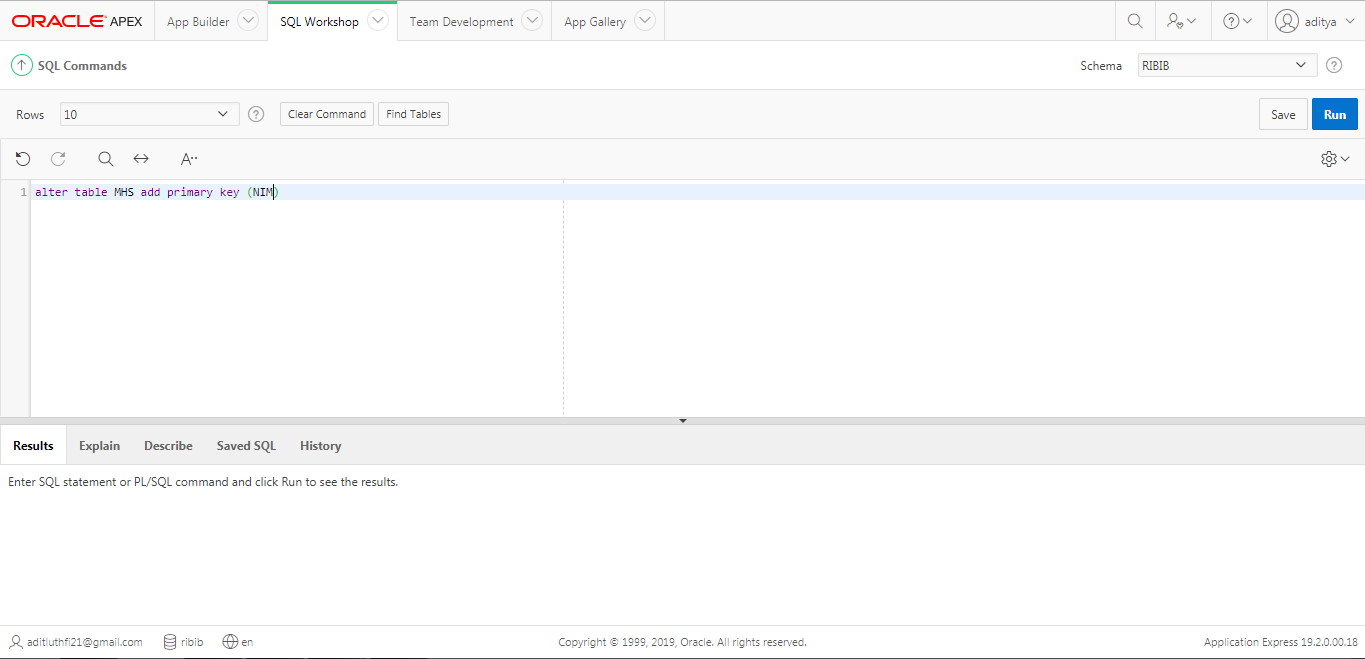
\includegraphics[width=.8\textwidth]{11.PNG}
\end{center}
\section{Lalu Run Application}
\begin{center}
    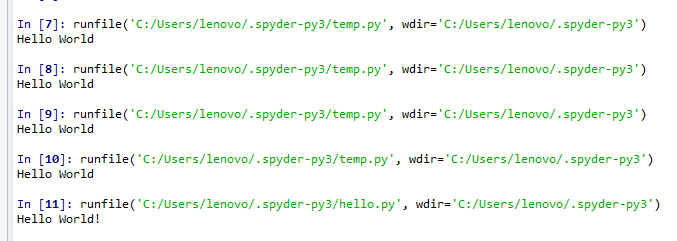
\includegraphics[width=.8\textwidth]{12.PNG}
\end{center}
\section{Masukkan lagi Username dan Password}
\begin{center}
    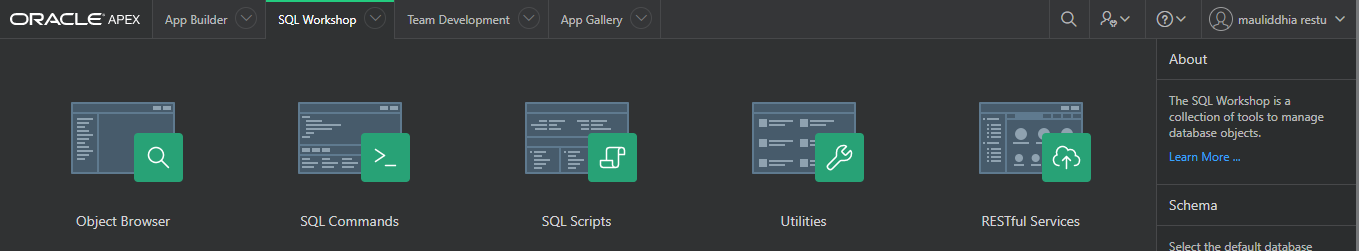
\includegraphics[width=.8\textwidth]{13.PNG}
\end{center}
\section{Pada Laman berikutnya klik Mahasiswa Search}
\begin{center}
    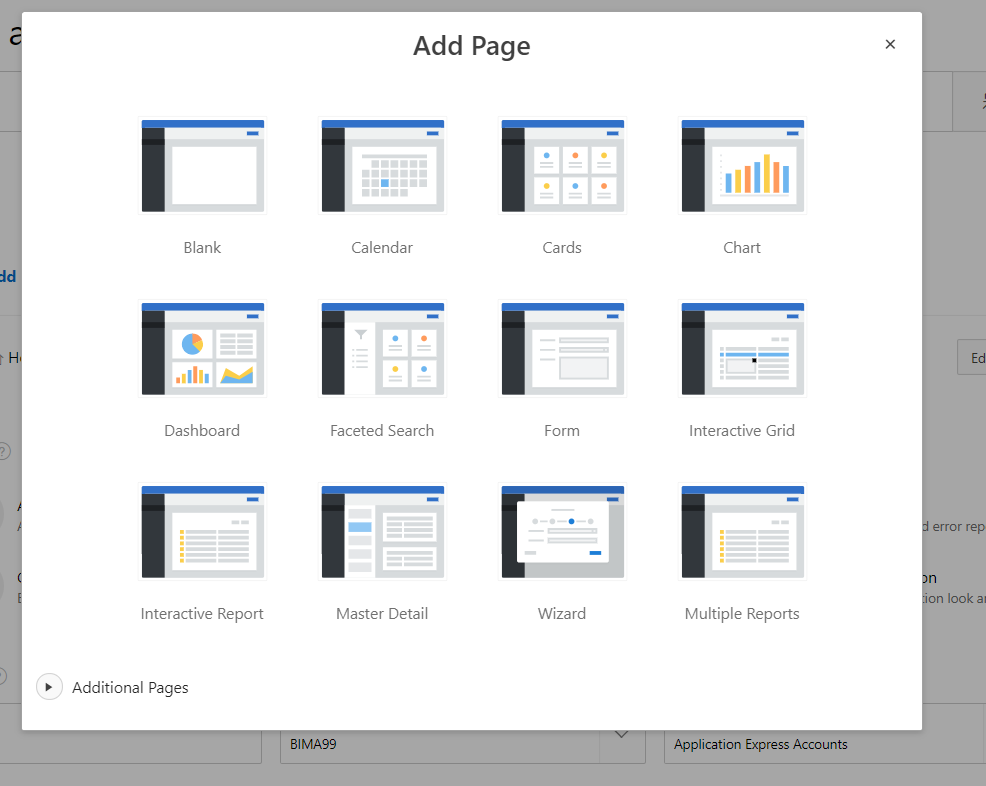
\includegraphics[width=.8\textwidth]{14.PNG}
\end{center}
\section{Maka akan terlihat tampilan data }
\begin{center}
    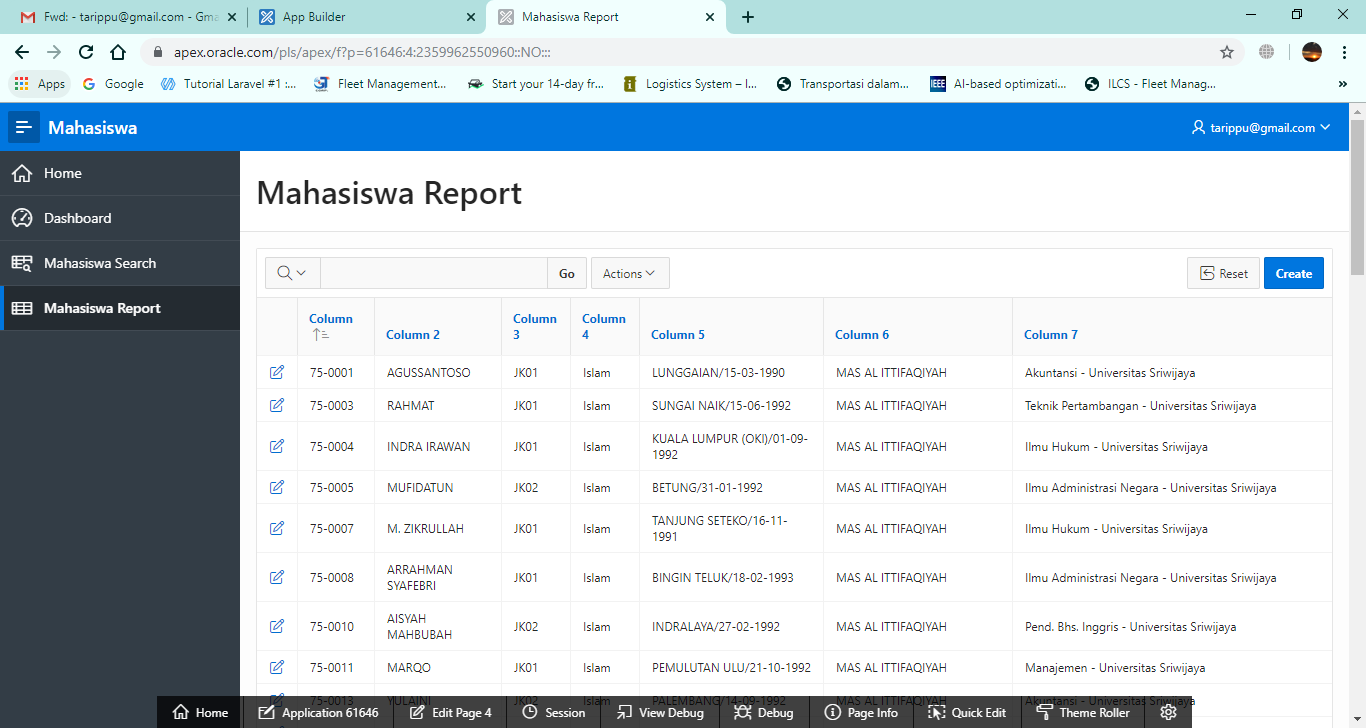
\includegraphics[width=.8\textwidth]{16.PNG}
\end{center}

\end{document}
